\chapter{Especificação técnica} \label{cap:especificacao_tecnica}
Neste capítulo são apresentadas as especificações do sistema, as condições restritivas, benefícios e impactos, análise funcional e de requisitos, a arquitetura do sistema e seus custos.

\section{Análise de Contexto}

    O desenvolvimento deste protótipo tem a finalidade de auxiliar o professor no ensino de programação para crianças.
    
    \subsection{Visão Geral}
    
    O software, apresentado em forma de jogo com o tema reciclagem, apresentará diversos desafios em que a criança deverá solucionar criando sequências lógicas com blocos físicos. Após a ordenação dos blocos, de maneira em que achar correta, pela criança, ela deverá tirar fotos da sua solução e submetê-la para a avaliação do desafio dentro do aplicativo.
    
    Ao finalizar a captura da solução proposta, o aplicativo enviará a sequência de imagens para um servidor, hospedado na nuvem, o qual fará a análise das imagens dos blocos por meio de visão computacional a fim de identificar e converter os blocos em ações para o jogo.
    
    Ao final da conversão, o servidor devolverá para o jogo a solução proposta em ações.
    Caso a solução esteja correta, a criança passará para o próximo desafio, caso contrário, será oferecido uma nova tentativa.
    
    O aplicativo coletará dados durante o desafio para o preenchimento de relatórios que serão apresentados para o professor ou tutor através de um portal.
    
    A Figura \ref{figura:diagrama_blocos} apresenta a visão geral do sistema proposto.
  
    \begin{figure}[H]
        \caption{Visão geral do sistema}
        \centering
        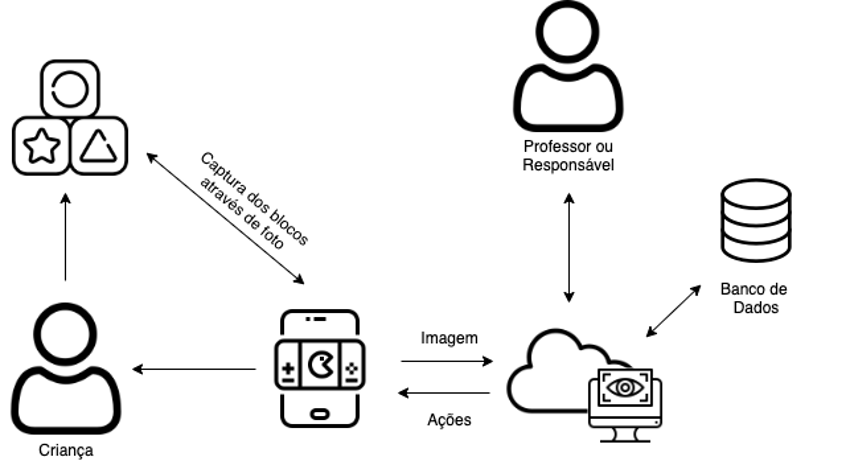
\includegraphics[width=\linewidth]{Imagens/cap3/diagrama_blocos.png}
        \legend{\small{Fonte: o autor (2020)}}
        \label{figura:diagrama_blocos}
    \end{figure}
    
    \subsection{Condições Restritivas}
    O projeto proposto apresenta algumas condições restritivas, conforme descrito nos próximos subitens.

        \subsubsection{Custos}
        Apesar do aplicativo jogo precisar de materiais relativamente baratos para ser jogado, como blocos impressos em 3D ou até mesmo papéis coloridos dobrados de forma semelhante aos blocos impressos, ainda se faz necessário o uso de um celular com sistema operacional Android com câmera para que o aplicativo funcione. 
            
        \subsubsection{Físicas e Ambientais}
        Apesar, quando impressos em 3D, dos bloco terem uma boa durabilidade, com o passar do tempo ficarão inutilizáveis. Portanto deve-se orientar os usuários do aplicativo jogo a fazer o descarte adequado dos blocos físicos depois de inutilizáveis, seja por desgaste dos blocos ou por falta de uso, o que vai de encontro com uma das propostas levantada pelo aplicativo jogo, a reciclagem.
        
        \subsubsection{Tecnológicas}
        O aplicativo jogo necessita de um celular com câmera e com o sistema operacional Android com a versão igual ou superior a 5.0 - Lollipop. Por se tratar de um protótipo, o aplicativo não oferece suporte para os demais dispositivos móveis com outros sistemas operacionais, como por exemplo Iphones. 
        
        \subsubsection{Energização}
        O celular é limitado em relação à energia, tendo um período máximo que uma carga pode sustentar, esse período máximo varia conforme o modelo e o uso do dispositivo. Para diminuir os efeitos causado por essa limitação, recomenda-se o uso do aplicativo com a bateria cheia ou próximo a uma tomada caso seja necessário recarregar a bateria do dispositivo móvel.    
        
        \subsubsection{Interferências devido ao meio}
        O aplicativo jogo precisa de conexão com internet para funcionar. Obstáculos como objetos metálicos ou paredes podem causar interferências no sinal Wi-Fi. Eletrônicos e eletrodomésticos, como por exemplo micro-ondas, operam na mesma frequência do roteador wireless, 2,4 GHz, que quando ligados, também podem contribuir com interferências dificultando ou até impossibilitando o uso do aplicativo.
    
    \subsection{Benefícios e Impactos}
    O aplicativo jogo apresenta alguns benefícios e impactos, conforme descrito nos próximos subitens.

        \subsubsection{Econômicos}
        Além de um celular com câmera, o aplicativo jogo proposto é capaz de funcionar com recursos relativamente baratos, como blocos impressos em 3D ou até mesmo uma folha colorida dobrada em formatos semelhantes aos cubos; o aplicativo jogo também funciona de forma simples. Portanto pode ser utilizado em casa ou implantado em escolas de forma fácil e econômica para proporcionar a crianças um contato inicial com temas como lógica de programação e sustentabilidade, além de atender às novas demandas da BNCC para o ensino.
        
        \subsubsection{Operacionais}
        O aplicativo jogo pode ser aplicado em ambiente escolar. Por ser uma ferramenta que difere dos métodos tradicionais de ensino das escolas, pode ser uma experiência lúdica o que impacta diretamente na rotina das crianças.
        
        \subsubsection{Estratégicos}
        A mais nova atualização da Base Nacional Comum Curricular destina uma de suas dez competência à educação integral por meio de tecnologias digitais e faz uso, no caderno de matemática, do termo “pensamento computacional”. Pensando nisso, o aplicativo jogo proposto possibilita, de uma forma estratégica, um meio para trabalhar essas competências nas escolas. 
        
        \subsubsection{Políticos}
        Não se aplica.

        \subsubsection{Sociais}
        O aplicativo jogo apresenta benefícios sociais para as crianças, pois as crianças terão acessos a conceitos básicos de lógica de programação e oportunidade de exercitar esse conceitos, o que pode auxiliar em competências como raciocínio lógico, resolução de problemas, pensamento computacional, entre outras habilidades que tem sido cada vez mais requisitadas no mercado de trabalho. 
        Isso sendo proporcionado por um jogo, além de gerar maior engajamento no ensino de crianças, pode desenvolver, também, competências como cooperação, cumprimento de regras, controle de impulsividade, auxílio na tomada de decisões, mais facilidade para lidar com erros e fracassos entre outras habilidades sociais.
        Além disso, o aplicativo jogo, por meio do tema de reciclagem, pode desenvolver senso de sustentabilidade auxiliando na compreensão da importância do descarte correto do lixo, o que impacta direta e positivamente  o meio ambiente.

\section{Análise Funcional e de Requisitos Tecnológicos}
    Nessa sessão, é apresentada a análise funcional e os requisitos tecnológicos do sistema.

    \subsection{Lista de Funcionalidade e Atores}
    O sistema será composto  pelas seguintes funcionalidades:
    \begin{itemize}
        \item Desafios de lógica com o tema reciclagem;
        \item Identificação dos blocos;
        \item Conversão dos blocos em ações;
        \item Relatórios de jogo para acompanhamento do professor.
    \end{itemize}
    
    O sistema tem como atores a criança e o professor/tutor.
    
    A criança é responsável pela interação com os blocos e aplicativo.
    O professor/tutor é responsável pela interação com os dados adquiridos durante a partida da criança.
    
    \subsection{Comunicação}
    A comunicação entre o aplicativo e o servidor ocorrerá de maneira bidirecional e utilizará arquitetura \textit{REST}, através da conexão Wi-Fi com a Internet.
    O aplicativo envia os dados e imagens para o servidor. Após o servidor salvar os dados e processar as imagens, ele retorna as ações a serem executadas para o aplicativo.
    
        \subsubsection{REST}
        O \textit{REST (Representational State Transfer)} é uma abstração da arquitetura da \textit{Web}. Consistem em regras que permitem a criação de projetos com interfaces bem definidas, permitindo a comunicação entre aplicações.
    
    \subsection{Processamento}
    O processamento por parte do Software, ocorre tanto no aplicativo quanto no servidor.
    O aplicativo captura as imagens e as envia para o servidor através da Internet.
    O servidor recebe as imagens enviadas pelo aplicativo e passa cada uma pelo algoritmo de visão computacional, responsável pela identificação de cada bloco nas fotos. Após a identificação dos blocos, é salvo a sequência no banco de dados e as ações são enviadas para o aplicativo.
    Após receber o retorno com as ações, o aplicativo transforma as ações em código e executa o mesmo durante o jogo.
    % Precisa escrever sobre o processamento das imagens, qual tipo de modelo, biblioteca, linguagem etc.
    
    \subsection{Interface Homem-Máquina}
    As interações da criança serão com os blocos físicos e com o aplicativo.
    Na tela inicial, são apresentadas duas opções, créditos e desafios, como mostra a Figura \ref{figura:tela_inicial}.
    
    \begin{figure}[H]
        \caption{Tela Inicial}
        \centering
        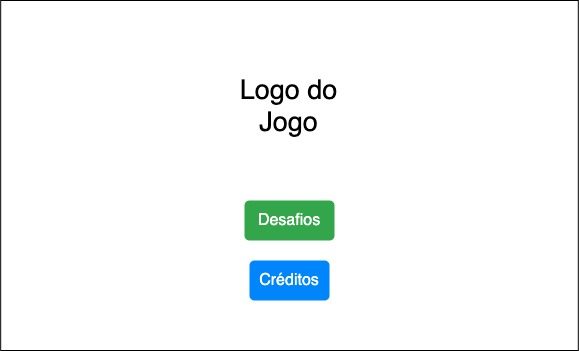
\includegraphics[width=\linewidth]{Imagens/cap3/Tela Inicial.jpg}
        \legend{\small{Fonte: o autor (2020)}}
        \label{figura:tela_inicial}
    \end{figure}
    
    Ao acessar a opção de desafios é apresentada a lista de todos os desafios disponíveis, juntamente com o progresso de cada desafio (se disponível), conforme apresentado na Figura \ref{figura:tela_desafios}.
    
    \begin{figure}[H]
        \caption{Tela de Desafios}
        \centering
        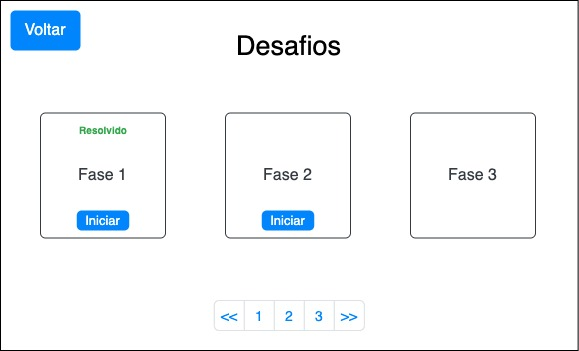
\includegraphics[width=\linewidth]{Imagens/cap3/tela_desafios.jpg}
        \legend{\small{Fonte: o autor (2020)}}
        \label{figura:tela_desafios}
    \end{figure}
    
    Nessa tela, é possível ver a lista de desafios, um desafio só poderá ser iniciado caso o anterior tenha sido resolvido.
    É possível clicar no botão voltar para retornar à tela anterior.
    Ao clicar no botão iniciar do desafio, a criança poderá ser direcionada para a tela de cadastro ou direto para a tela do desafio.
    Caso a criança não tenha preenchido as informações para identificá-la, essas informações serão coletadas em uma tela específica, conforme Figura \ref{figura:cadastro}. Caso contrario ela é direcionada para a tela que contém o desafio a ser solucionado.
    
    \begin{figure}[H]
        \caption{Tela de Cadastro}
        \centering
        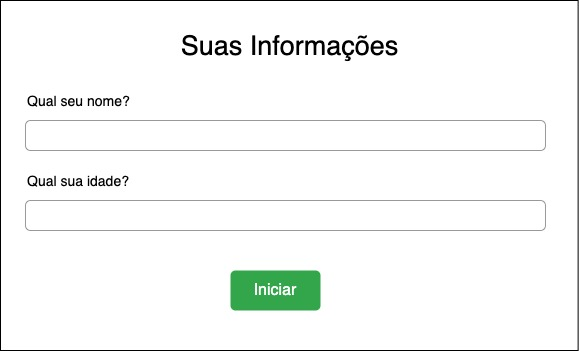
\includegraphics[width=\linewidth]{Imagens/cap3/informacoes_usuario.jpg}
        \legend{\small{Fonte: o autor (2020)}}
        \label{figura:cadastro}
    \end{figure}
    
    A Figura \ref{figura:tela_jogo} mostra a interface principal durante o jogo.
    
    \begin{figure}[H]
        \caption{Tela do Jogo}
        \centering
        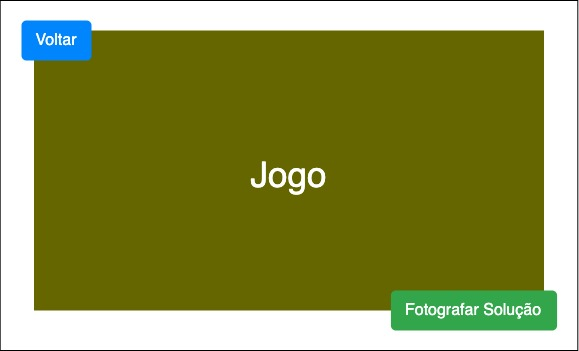
\includegraphics[width=\linewidth]{Imagens/cap3/tela_jogo.jpg}
        \legend{\small{Fonte: o autor (2020)}}
        \label{figura:tela_jogo}
    \end{figure}
    
    Nessa tela é possível executar duas ações.
    Clicando no botão voltar, a criança é redirecionada para a lista de desafios.
    Selecionando o botão Fotografar Solução, é aberto uma janela, conforme Figura \ref{figura:fotografar_blocos} para fotografar a solução.
    
    \begin{figure}[H]
        \caption{Tela para fotografar a solução}
        \centering
        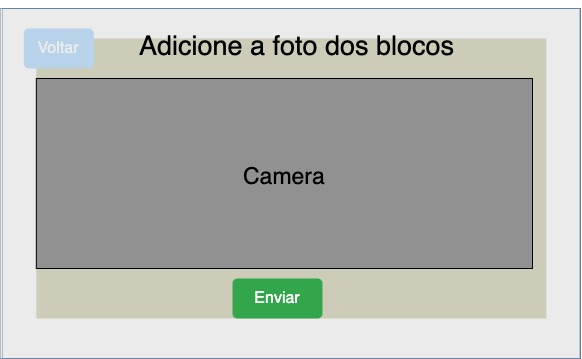
\includegraphics[width=\linewidth]{Imagens/cap3/UploadSolucao.jpg}
        \legend{\small{Fonte: o autor (2020)}}
        \label{figura:fotografar_blocos}
    \end{figure}
    
    Cada bloco deve ser fotografado e adicionado utilizando o botão Novo Bloco.
    Ao fotografar todos os blocos, pode-se clicar no botão enviar para que a solução seja processada.
    Após a conversão das fotos em ações para o jogo, o usuário é direcionado para a tela de jogo, onde as ações convertidas serão executadas.
    Caso a solução seja a correta e o personagem chegue na lixeira correta, será apresentado uma mensagem de sucesso, conforme Figura \ref{figura:solucao_correta}. Caso contrário, será apresentado a mensagem de falha, permitindo uma nova tentativa, Figura \ref{figura:solucao_incorreta}.
    
    \begin{figure}[H]
        \caption{Mensagem de solução correta}
        \centering
        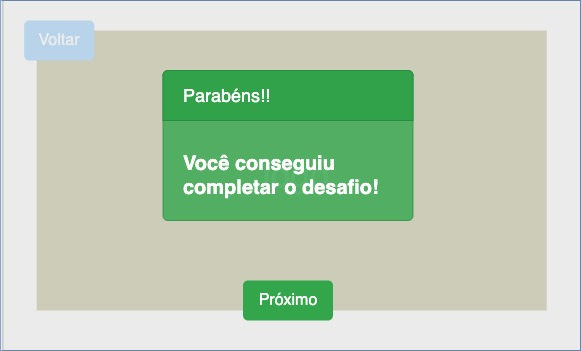
\includegraphics[width=\linewidth]{Imagens/cap3/solucao_correta.jpg}
        \legend{\small{Fonte: o autor (2020)}}
        \label{figura:solucao_correta}
    \end{figure}
    
    \begin{figure}[H]
        \caption{Mensagem de solução incorreta}
        \centering
        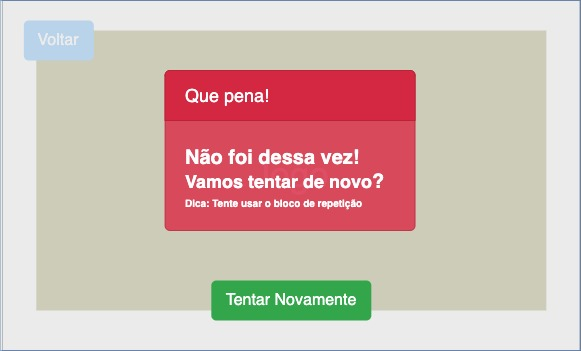
\includegraphics[width=\linewidth]{Imagens/cap3/solucao_incorreta.jpg}
        \legend{\small{Fonte: o autor (2020)}}
        \label{figura:solucao_incorreta}
    \end{figure}
    
    
    \subsection{Sistemas Controlados Automaticamente}
    O Sistema não apresentará sistemas controlados automaticamente.
    
    \subsection{Aquisição de dados e Atuação}
    A coleta das fotos se dará através da ação da criança que está jogando. Após concluir a proposta de solução do desafio, a mesma deve capturar sua proposta utilizando a câmera do dispositivo móvel, como mostrado na Figura \ref{figura:crianca_blocos}
    
    \begin{figure}[H]
        \caption{Criança capturando a solução}
        \centering
        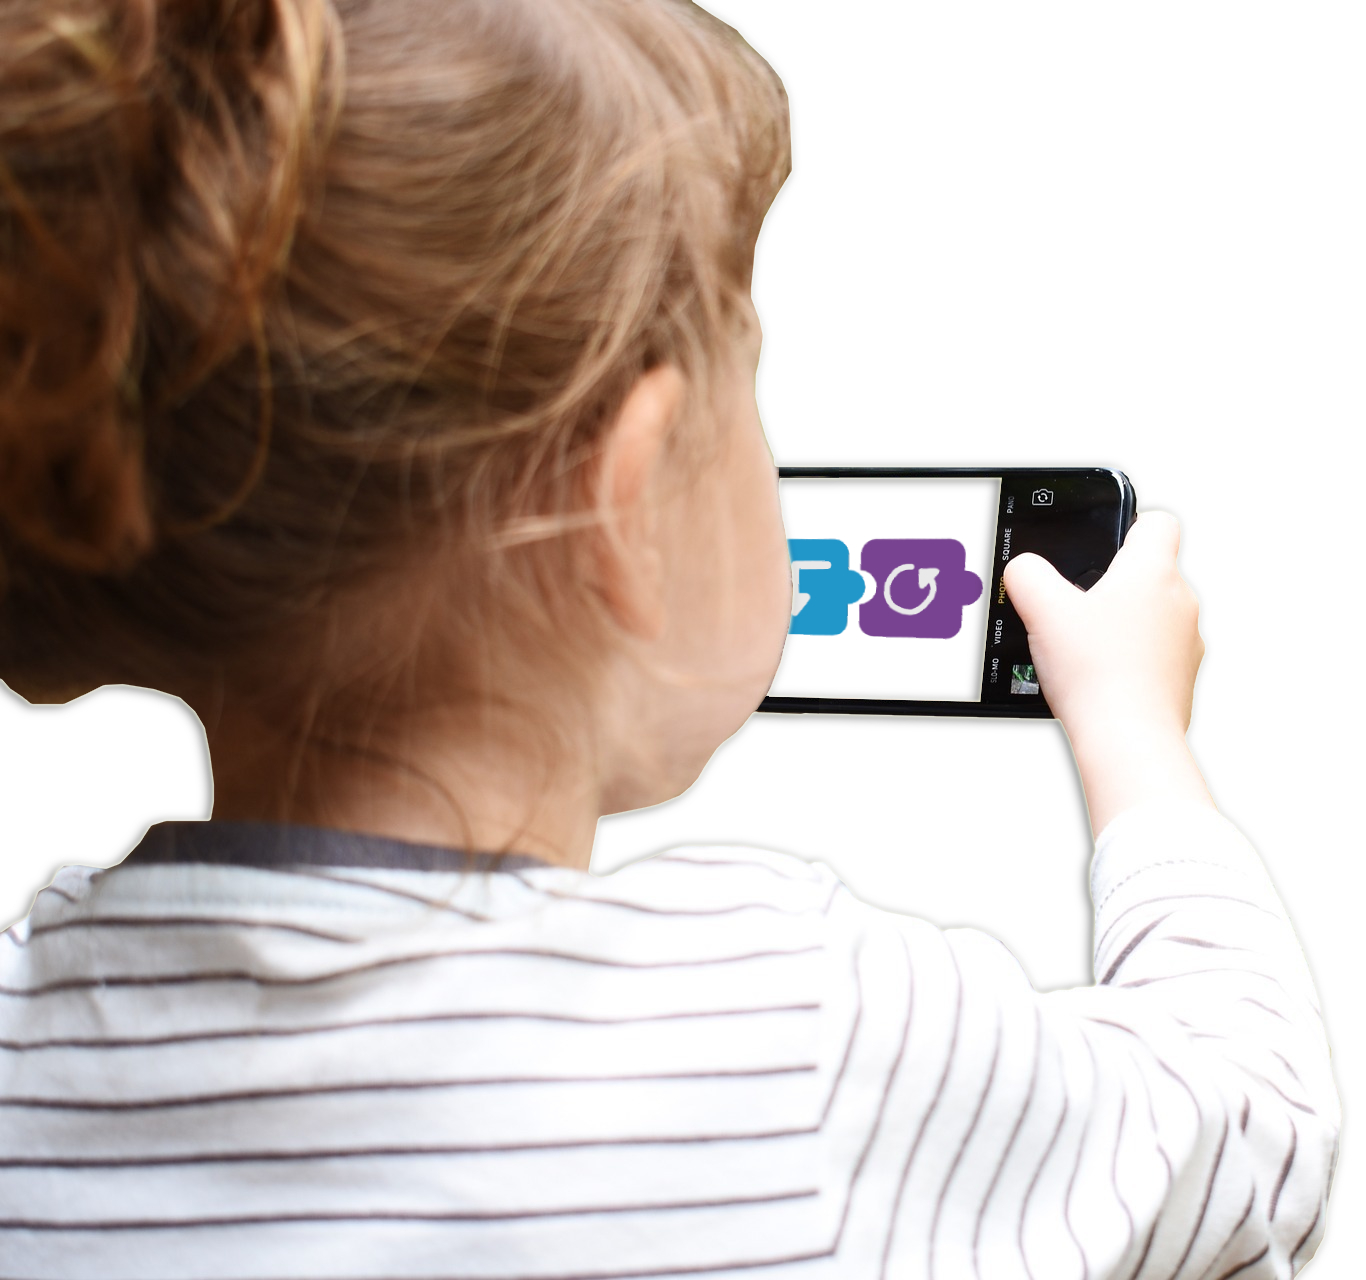
\includegraphics[width=10cm]{Imagens/cap3/CriançaBlocos.jpg}
        \legend{\small{Fonte: o autor (2020)}}
        \label{figura:crianca_blocos}
    \end{figure}
    
    Após a captura da imagem, a criança, utilizando um botão de envio, enviará a foto para o servidor, onde ela será e transformada em ações para o jogo.
    
    O envio da foto e o recebimento da conversão em ações do jogo é realizado através de conexão com a Internet.
    Toda proposta de solução, esteja ela correta ou não, será salva no banco de dados, após sua interpretação, para gerar relatórios estatísticos.


\section{Análise da Arquitetura do Sistema}
    Nessa sessão, são apresentadas as arquiteturas de hardware e software do sistema.

    \subsection{Hardware}
    O hardware do sistema será composto por blocos físicos e o dispositivo mobile com câmera.
    
    O dispositivo mobile deverá ser um celular \textit{Android} com câmera, podendo variar entre os modelos existentes no mercado.
    
    Os blocos físicos serão construídos de PLA, impressos em 3D, com o tamanho aproximado de 10cm x 10cm x 5mm, seus cantos serão arredondados para evitar acidentes no manuseio. Para facilitar a identificação, além da sua cor, cada bloco possuirá um simbolo representado o tipo da ação conforme mostrado na Figura \ref{figura:blocos_fisicos}.
    
    \begin{figure}[H]
        \caption{Blocos Físicos}
        \centering
        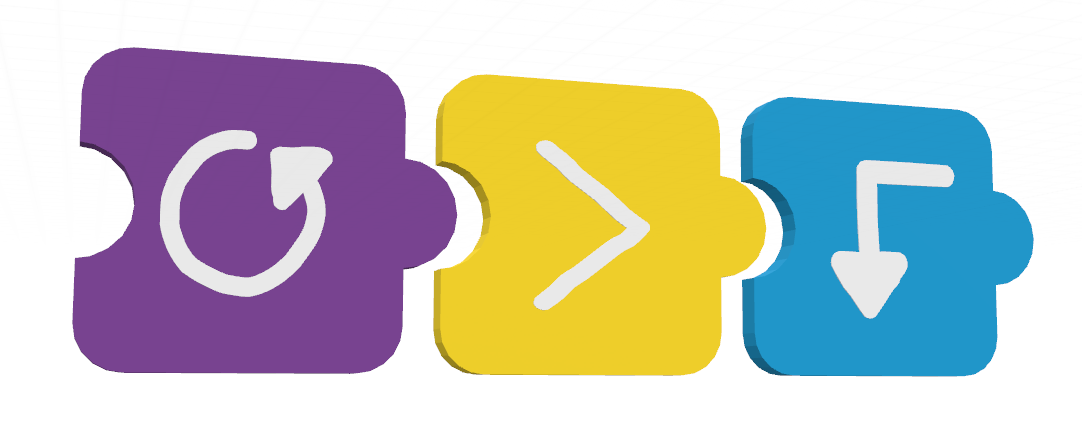
\includegraphics[width=\linewidth]{Imagens/cap3/Blocos.png}
        \legend{\small{Fonte: o autor (2020)}}
        \label{figura:blocos_fisicos}
    \end{figure}
    
    As ações são divididas em dois tipos, que são apresentados nos próximos tópicos.
    
        \subsubsection{Ações Diretas}
        As ações diretas são andar, apresentado na Figura \ref{figura:andar}, e girar 90 graus, apresentado na Figura \ref{figura:girar}. Ao identificar esse bloco, o código irá executar a ação escolhida.
        
        \begin{figure}[H]
            \caption{Andar}
            \centering
            
\includegraphics[width=5cm]{Imagens/cap3/Ande.png}
            \legend{\small{Fonte: o autor (2020)}}
            \label{figura:andar}
        \end{figure}
        
        \begin{figure}[H]
            \caption{Gire 90 graus}
            \centering
            
\includegraphics[width=5cm]{Imagens/cap3/Gire.png}
            \legend{\small{Fonte: o autor (2020)}}
            \label{figura:girar}
        \end{figure}
        
        \subsubsection{Ação de Repetição}
        A ação de repetição, mostrada na Figura \ref{figura:repita}, possibilitará uma otimização do código, visto que, ao identificar esse bloco, criará um loop e executará as ações contidas entre dois blocos conforme mostra a Figura \ref{figura:repita_exemplo}.
        
        \begin{figure}[H]
            \caption{Repita}
            \centering
            
\includegraphics[width=5cm]{Imagens/cap3/Repita.png}
            \legend{\small{Fonte: o autor (2020)}}
            \label{figura:repita}
        \end{figure}
        
        \begin{figure}[H]
            \caption{Exemplo para repetição}
            \centering
            \includegraphics[width=\linewidth]{Imagens/cap3/repita_exemplo.png}
            \legend{\small{Fonte: o autor (2020)}}
            \label{figura:repita_exemplo}
        \end{figure}
    
    \subsection{Software}
    A arquitetura do software será baseada em serviços cloud e mobile. Para o ambiente cloud, será utilizado a IBM Cloud como provedor.
    O servidor, programado em Python, utilizará um serviço \textit{PAAS (Platform as a Service)} chamado Cloud Foundry. O banco de dados, não relacional, utilizará o serviço IBM Cloudant desenvolvido no Apache CouchDB que utiliza JSON para armazenar os dados.
    
    Nos tópicos a seguir, são apresentadas as ferramentas de desenvolvimento e os diagramas do software que representam o seu funcionamento.
        
        
        \subsubsection{Ferramentas de Desenvolvimento}
        
        Na etapa de desenvolvimento do reconhecimento da imagem dos blocos será utilizado o Jupyter Notebook como ambiente de desenvolvimento juntamente com a linguagem de programação Python versão 3. Os módulos para visão computacional e aprendizado de máquina serão OpenCV, TensorFlow, Keras entre outros. As principais ferramentas estão descritas abaixo.
        
    
            \subsubsubsection{Jupyter Notebook}
    
            O Jupyter notebook foi criado em 2014, sem objetivos lucrativos, como uma extensão do IPython, o jupyter tem o propósito de ter suporte para várias linguagens de programação para o desenvolvimento iterativo da computação científica e da ciência dos dados. O jupyter possui uma interface chamada Notebook, esta interface é executada diretamente no navegador web e possibilita a integração entre  execuções de códigos, gráficos, textos, imagens, vídeos e diversas outras formas de visualizações suportada pelos navegadores atuais. Outro recurso do Notebook é o compartilhamento do arquivo .ipynb de forma simples e em diversos formatos, como por exemplo HTML, pdf, entre outros.
            
        	O jupyter também possui, juntamente com o código, suporte para a linguagem de marcação textual Markdown, desta forma o jupyter possibilita a criação de relatórios, guias e documentações com grande qualidade visual.  Por conta disso e pela facilidade de visualização dos processos e resultados, o Jupyter Notebook foi escolhido como interface para o desenvolvimento em Python. 
                
            \subsubsubsection{Python}
            A linguagem de programação Python foi desenvolvida em 1989 por Guido Van Rossum. Rossum tinha o objetivo de desenvolver uma linguagem capaz de agilizar processos de criação de softwares. 
        	O Python é uma linguagem de alto nível e interpretada, usada de maneira Interativa e Scripts. Hoje companhias como Google, Yahoo, CERN e Nasa utilizam Python em suas aplicações. Por sua ampla utilização e baixa complexidade, diversos programadores desenvolvem pacotes, conhecidos na linguagem como módulos, que estendem o horizonte de aplicação da linguagem. Por conta de módulos como Scikit learning, Numpy, desenvolvidos na academia, que facilitam operações com vetores, o Python se tornou bastante utilizado em aplicações com inteligência artificial,  principalmente na academia.
        	
            Além de Inteligência artificial, a linguagem Python também é utilizada em aplicações web, análise e visualização de dados, desenvolvimento de jogo, sistemas embarcados, entre outras. Por conta de sua ampla aplicabilidade e baixa complexidade,  é uma das linguagens de programação mais utilizadas hoje em dia e possui uma das comunidades mais ativas em fóruns, eventos e cursos. Devido a esses fatores, Python foi escolhido para o desenvolvimento desta etapa do aplicativo jogo.  
                
            \subsubsubsection{OpenCV}
            O OpenCV consiste em uma plataforma com diversa bibliotecas para o desenvolvimento de aplicações de Aprendizado de Máquinas e Visão Computacional. A plataforma OpenCV foi desenvolvida pela Intel com o propósito de oferecer uma infraestrutura universal para aplicações de Visão Computacional tanto no mercado quanto acedemia. O OpenCV possui mais de 2.500 algoritmos para detecção de faces, identificação de objetos, classificação de ações e objetos em imagens e vídeos, entre outras aplicações de Visão Computacional.
            
            O OpenCV possui suporte para C++, Java, Python, linguagem M e pode ser usado em sistemas operacionais como Android, Windows, Mac, Linux. Empresas como Google, Microsoft, Intel, Honda,  IBM fazem uso da plataforma OpenCV. Pela relevância na academia e quantidade de algoritmos de visão computacional que o OpenCV possui, esse pacote foi escolhido como módulo base para visão computacional nessa aplicação.
            
            \subsubsubsection{TensorFlow e Keras}
             O TensorFlow foi desenvolvidos por pesquisadores do Google com o objetivo de produzir uma interface de aprendizado de máquina que teria a capacidade de ser executada, da mesma forma, tanto em em grandes servidores de GPUs quanto pequenas aplicações mobile. O tensorflow é um módulo com código aberto para execução de algoritmos aprendizado de máquinas. Como outras ferramentas citadas acima, é utilizado tanto pela comunidade científica quanto por profissionais da indústria.
             
            O TensorFlow é usado para inferência e treinamento de modelos de Deep Learning. Portanto pode ser usado em aplicações de processamento de linguagem natural, visão computacional, robótica, entre outras.
            
            O Keras funciona como uma camada de alto nível sobre o TensorFlow, o que facilita a programação de algoritmos de Deep Learning. Hoje o Keras está integrado como um módulo ao TensorFlow.  
            
            \subsubsubsection{Unity}
    
            O Unity foi criado em 2005 por David Helgason, Joachim Ante e Nicholas
            Francis na Dinamarca. É uma ferramenta com bastante força no mercado de jogos por suportar o desenvolvimento para diversas plataformas digitais. 50\% dos jogos entre todas as plataformas são feitos usando Unity tendo mais de 3 bilhões de dispositivos alcançados no mundo todo \cite{dados_unity}.
            
            Muitos jogos criados no Unity alcançaram sucesso de vendas e se tornaram bastante conhecidos, por exemplo o jogo Cuphead, criado pelo StudioMDHR lançado em 2017 para as plataformas Xbox One, Windows 10, e Steam \cite{cuphead}. Outro jogo bastante conhecido é o Monument Valley 2 lançado em 2017 para as plataformas Android e IOS\cite{monument_valley_2}.

    
       \subsubsection{Banco de Dados de Imagens}    
        
        Para o desenvolvimento da etapa de reconhecimento, será desenvolvida uma base de dados de imagens para treinamento da rede. As imagens serão dos próprio blocos físicos impressos em 3D e de blocos impressos em papel e dobrados de forma semelhante aos blocos em 3D.	As imagens serão capturadas por meio de um dispositivo celular com câmera, semelhante ao que será utilizado pelo usuário durante o uso do aplicativo jogo, em diferentes posições, ambientes e luminosidades. 
        
        A base possuirá diversas imagens por tipo de bloco. Ao todo será por volta de 1000 imagens dos blocos. As imagens da base serão em resolução 1920x1080, isto é, Full HD, e em formato PNG (Portable Network Graphics). Em média cada arquivo terá 4MB. Cada imagem terá uma identificação correspondente ao seu bloco. 

        \subsubsection{Serviços Cloud}
        \subsubsubsection{Cloud Foundry}
        \subsubsubsection{Cloudant}
        
        \subsubsection{DER/MER}
        O diagrama apresentado na Figura \ref{figura:der_mer} mostra os relacionamentos entre os esquemas do sistema, crianca e resolucao\_desafio, juntamente com seus atributos, nome, idade, numero, tempo, está correta e blocos.
        
        \begin{figure}[H]
            \caption{Diagrama Entidade Relacionamento}
            \centering
            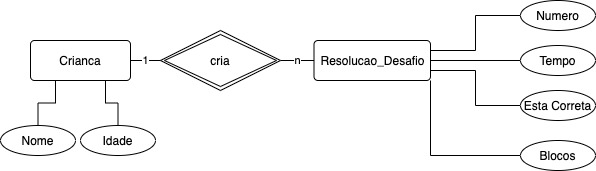
\includegraphics[width=\linewidth]{Imagens/cap3/MER_DER.jpg}
            \legend{\small{Fonte: o autor (2020)}}
            \label{figura:der_mer}
        \end{figure}
        
        O banco de dados possuirá dois esquemas de documentos, um para representar a criança e outro para representar a resolução do desafio.
        O esquema da criança, possui obrigatoriamente os atributos de Nome e Idade.
        O esquema para a resolução do desafio, possui os seguintes atributos:
        
        \begin{itemize}
            \item Numero, representando o número do desafio.
            \item Tempo, representando o tempo que a criança levou para submeter a solução.
            \item Esta Correta, representando se a solução apresentada está correta ou não.
            \item Blocos, representando os blocos que foram utilizados.
        \end{itemize} 
        
        \subsubsection{Use Case}
        O Aplicativo conta com funções de identificação da criança (Perfil), Inicio de desafio e submissão de solução, conforme apresentado no diagrama de caso de uso na Figura \ref{figura:use_case}.
        
        \begin{figure}[H]
            \caption{Use Case}
            \centering
                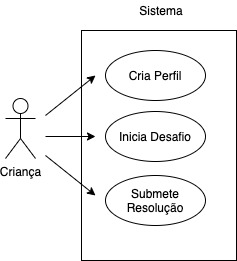
\includegraphics[width=10cm]{Imagens/cap3/Use Case.jpg}
    
            \legend{\small{Fonte: o autor (2020)}}
            \label{figura:use_case}
        \end{figure}
        
        \subsubsection{Diagramas de Sequência}
        
        Nesse tópico são apresentados os diagramas de sequencia para as funcionalidades principais do aplicativo.
        
        \subsubsubsection{Criação de Perfil}
        
        A Figura \ref{figura:sequencia_perfil} mostra o diagrama de sequência para a realização do cadastro de informações da criança. Todas as informações são salvas localmente e em um banco de dados na nuvem.
        
        \begin{figure}[H]
            \caption{Diagrama de Sequência - Perfil}
            \centering
                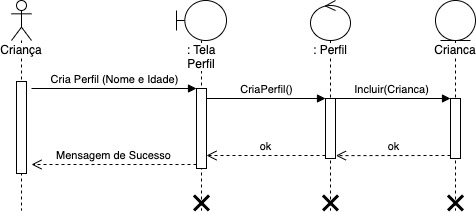
\includegraphics[width=\linewidth]{Imagens/cap3/Sequencia_Perfil.jpg}
    
            \legend{\small{Fonte: o autor (2020)}}
            \label{figura:sequencia_perfil}
        \end{figure}
        
        \subsubsubsection{Submissão da Resolução}
        
        O diagrama apresentado na Figura \ref{figura:sequencia_jogo} mostra o processo de submissão da solução e validação da mesma.
        
        \begin{figure}[H]
            \caption{Diagrama de Sequência - Submissão da Resolução}
            \centering
                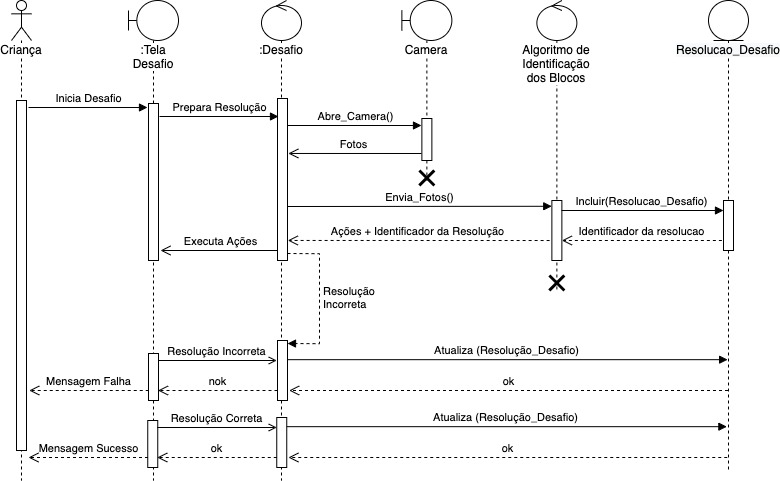
\includegraphics[width=\linewidth]{Imagens/cap3/Sequencia_Jogo.jpg}
    
            \legend{\small{Fonte: o autor (2020)}}
            \label{figura:sequencia_jogo}
        \end{figure}
        
        Ao iniciar o desafio, a data e hora são salvos localmente para que, quando a resolução for submetida, essa informação seja salva junto com as demais no banco de dados. Após o aplicativo processar as ações convertidas pelo algoritmo de identificação dos blocos, o aplicativo valida a solução e atualiza a resolução no banco com o seu status, correto ou não correto.
        
        \subsubsubsection{Visualização de Relatório}
        
        O diagrama apresentado na Figura \ref{figura:sequencia_tutor} mostra o processo para o tutor visualizar os relatórios dos desafios submetidos pelas crianças.
        
        \begin{figure}[H]
            \caption{Diagrama de Sequência - Visualização de Relatorio}
            \centering
                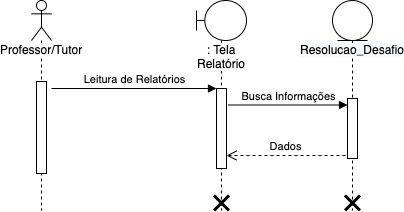
\includegraphics[width=\linewidth]{Imagens/cap3/sequencia_tutor.jpg}
            \legend{\small{Fonte: o autor (2020)}}
            \label{figura:sequencia_tutor}
        \end{figure}